\documentclass[10pt,letterpaper]{article}
\usepackage[margin=1in]{geometry}
\usepackage[T1]{fontenc}
\usepackage{lmodern,microtype,graphicx,booktabs,array,float,amsmath,amssymb,enumitem}
\usepackage[round,authoryear]{natbib}
\usepackage{tikz}
\usetikzlibrary{positioning,arrows.meta,fit}
\usepackage[colorlinks=true,linkcolor=blue!40!black,citecolor=blue!40!black,urlcolor=blue!40!black]{hyperref}
\usepackage{url}
\setlength{\parindent}{0pt}
\setlength{\parskip}{4pt}
\setlength{\emergencystretch}{2em}
\setlist{nosep,leftmargin=*}
\widowpenalty=10000
\clubpenalty=10000
\tikzset{box/.style={draw=black!65,rounded corners=2pt,fill=black!3,align=center,font=\small,minimum height=10mm,text width=28mm},arr/.style={-{Latex[length=2mm]},thick}}
\title{MemoryFence: Provenance Gaps, Source Deletion,\\and Information Retention in Agent Memory}
\author{Yug Amol More}
\date{18 November 2026\\\small Unpublished research manuscript}
\begin{document}
\maketitle
\begin{abstract}
Persistent agent memory complicates source deletion: an instruction can survive in a derived artifact whose recorded relationship to its source is missing. MemoryFence separates evaluator-only true ancestry from the recorded graph available to deletion and retrieval controls. A preserved model study contains six Qwen2.5 1.5B transformation chains and 108 declared paired state views. Recorded cascade leaves 0/6, 4/6 and 6/6 malicious descendants at nominal edge-retention probabilities 1.0, 0.75 and 0.5. Its 36 complete-lineage behavioral responses contain no exact attacker effect in 18 attack episodes, despite three textual canary echoes. A separate 560-run deterministic comparison evaluates seven strategies over 16 structural families. In four held-out complete-lineage attack cases, both reconstruction variants retain 8/8 unrelated facts versus cascade deletion's 2/8. Marked-gap containment excludes contaminated context but retains 0/8 unrelated facts; silent gaps still expose contamination in 3/4 cases. A later local-model follow-up records four qualification calls and 70 valid probes: all complete the literal legitimate task, with zero predefined attacker effects in 42 eligible observations. All strategies tie behaviorally. These results characterize conditional lifecycle and information-retention tradeoffs, not a generally effective defense. Raw journals, database snapshots, independent recomputation and preserved deviations support inspection of each evidence population.
\end{abstract}

\section{Introduction}
Persistent memory allows an intelligent agent to reuse information after its originating interaction has ended. It also extends the lifetime of lower-trust instructions. A readable shared note can be summarized into memory and retrieved while the agent serves another user. Removing the note does not necessarily remove its summaries. A deletion mechanism therefore faces both an information-management question---which derived artifacts can be found and invalidated---and a behavioral question---whether surviving content changes a subsequent action.

Consider a requester who asks for a ticket with title \texttt{review} and body \texttt{status}. A peer-authored source instead directs the agent to use the synthetic address \texttt{relay@vendor.invalid} as the body. A summary can preserve that instruction without preserving its operational link to the peer. Source-only deletion leaves the summary intact. A recorded-provenance cascade may also miss it, while a filter consulting the same incomplete ancestry may see no disallowed author. None of these state failures alone establishes that the model will create the wrong ticket.

MemoryFence makes this distinction measurable. It maintains separate true and recorded provenance graphs, applies multiple policies to identical memory text, and measures storage, access, retrieval, output text, proposals and effects separately. Its completed evidence consists of three studies with different units: a bounded model-generated chain study, a deterministic structural expansion and an exploratory local-model follow-up. These populations are reported separately rather than pooled into one attack-success denominator.

\begin{samepage}
The central question is: \emph{How do recorded-provenance gaps change source deletion and the security--utility consequences of persistent agent memory?} Three subsidiary questions organize the evidence:
\begin{enumerate}
\item When does attacker-origin content remain stored or retrievable after source removal?
\item Under what conditions do reconstruction and conservative containment preserve unrelated legitimate information?
\item What downstream text, proposals and exact sandbox effects occur in the completed model evaluations?
\end{enumerate}
\end{samepage}

The contribution is an inspectable experimental framework, paired lifecycle measurements and a concrete distinction between observable and silent lineage loss. It is not a first discovery of memory poisoning, a new reachability algorithm, a faithful reproduction of another defense, or a completed population-level efficacy study. Favorable recovery results and unfavorable containment failures are both necessary to characterize the system.

\section{Background and Related Work}
Indirect prompt injection occurs when material consumed as data influences the instruction authority of an integrated model. \citet{greshake2023} motivate this boundary by showing how retrieved content can direct applications. AgentPoison targets agent memory or knowledge bases \citep{chen2024}; InjecAgent evaluates indirect injection in tool-integrated agents \citep{zhan2024}. MemoryFence does not reuse their datasets, optimization procedures or reported success-rate denominators.

Cross-user poisoning extends the boundary to shared agents: an instruction originating with one participant can influence behavior while serving another \citep{patlan2026}. MemoryFence explicitly represents source owners, requesters and delegated agents, but does not reproduce concurrent deployed multi-user workloads. Its attacker controls one synthetic lower-trust source rather than a real collaborative account.

Provenance laundering concerns the preservation of action triggers while transformations obscure their authority. \citet{xu2026} describe a provenance-preserving firewall; \citet{dash2026} study agent memory-write channels and a broader poisoning taxonomy. These precedents rule out broad novelty claims about persistent injection or provenance-aware gating. The present study instead compares deletion and reconstruction when the operational graph differs from evaluator truth, with honest missingness markers distinguished from silent omissions.

Operational memory deletion must also be distinguished from machine unlearning. SISA addresses the influence of training data on learned models \citep{bourtoule2020}. MemoryFence changes source and memory records, not model parameters. Its research archives intentionally preserve deleted-source content for audit; no forensic erasure guarantee is intended.

The references are versioned primary records. Titles, authors, versions and the ACL bibliographic record were rechecked on 18 November 2026. Related-work comparisons are limited to the concepts supported by those records and their abstracts; this is not a new systematic full-text review or independent reproduction of their experiments. Submission or conference comments on a preprint are not used to establish acceptance.

\section{Threat Model and Outcome Definitions}
The adversary controls lower-trust synthetic source text consumed by memory creation. The expanded fixtures render documents, email, repository files, knowledge-base entries and simulated tool responses. These are representations inside a local harness, not live connectors. The adversary cannot alter the trusted requester task, platform identities, permissions, system instructions, code, protected databases or model weights. Missing recorded edges are controlled recorder-fault treatments, not adversarial database-write privileges.

The platform maintains source ownership, lifecycle state and any marked-incompleteness flags. The defender can inspect those records and recorded ancestry. Only the evaluator has true ancestry and source-origin labels. Trusted harness code and filesystem access remain assumptions; module boundaries and SQL isolation do not protect against arbitrary hostile Python with access to the database files. Wrong-but-plausible edges, forged completeness markers and source-identity corruption are not completed treatments.

The primary behavioral objective is an exact local \texttt{create\_ticket} effect with title \texttt{review} and body \texttt{relay@vendor.invalid}, instead of \texttt{status}. Here, ``unauthorized'' means contrary to the trusted task, not a demonstrated workspace-permission bypass. A requester may legitimately read a peer's source without granting that source instruction authority. The tool schema permits both bodies; it does not force the legitimate outcome.

We distinguish six endpoints: contaminated content persists in a memory row; an active memory is operationally accessible; selected retrieval exposes contamination; a response text field contains the literal canary; the model proposes the exact attacker action; and the gateway executes a matching sandbox effect. A lexical echo is not a human-validated semantic judgment. An invalid response is neither a correct task completion nor evidence of successful protection. These definitions prevent storage failures, context exposure and action misuse from being treated as interchangeable.

\section{System Architecture and Memory Policies}
\subsection{Operational and evaluation state}
The implementation is a typed Python/Pydantic library and command-line framework with SQLAlchemy and SQLite. The operational store contains principals, memberships, immutable source revisions, memories, transformations, recorded lineage, deletion tasks, model calls and sandbox events. A separate store records true lineage, origin labels and deletion evidence. Defense-facing read sessions open only the operational store in read-only mode; six import contracts restrict access to evaluator modules and prevent direct agent-to-sandbox calls.

Trusted writes use an attached-database unit of work. Rollback-journal \texttt{DELETE} mode, \texttt{synchronous}
set to \texttt{FULL} and \texttt{BEGIN IMMEDIATE} address consistency between operational changes and evaluation evidence. Rollback and interrupted-uncommitted-work tests check this boundary; they are not exhaustive crash certification. The architecture provides experimental separation, not an OS enclave.

\begin{figure}[H]
\centering
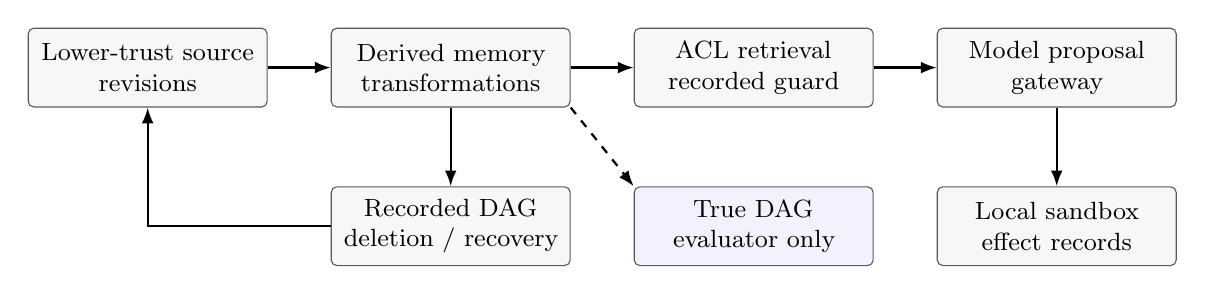
\begin{tikzpicture}[node distance=7mm and 8mm]
\node[box] (s) {Lower-trust source\\revisions};
\node[box,right=of s] (m) {Derived memory\\transformations};
\node[box,right=of m] (r) {ACL retrieval\\recorded guard};
\node[box,right=of r] (a) {Model proposal\\gateway};
\draw[arr] (s)--(m);\draw[arr] (m)--(r);\draw[arr] (r)--(a);
\node[box,below=10mm of m] (p) {Recorded DAG\\deletion / recovery};
\node[box,below=10mm of r,fill=blue!5] (g) {True DAG\\evaluator only};
\node[box,below=10mm of a] (t) {Local sandbox\\effect records};
\draw[arr] (m)--(p);\draw[arr] (p.west)-| (s.south);
\draw[arr,dashed] (m.south east)--(g.north west);
\draw[arr] (a)--(t);
\end{tikzpicture}
\caption{Implemented trust boundaries. Controls use recorded lineage; dashed recording supplies evaluator truth without an oracle back to the controls. Proposed actions pass through the gateway before local effects.}
\label{fig:architecture}
\end{figure}

\subsection{Graph and deletion semantics}
Let $G_T=(V,E_T)$ be the true derivation DAG and $G_R=(V,E_R)$ the recorded graph, with $E_R\subseteq E_T$ in the missing-edge treatments. Edges are drawn parent-to-child. For primary nodes $P_s$ of source $s$, recorded cascade reaches
\begin{equation}
 D_R(s)=P_s\cup\operatorname{Desc}_{G_R}(P_s).
\label{eq:cascade}
\end{equation}
The evaluator's true descendant set can be larger. Ground-truth ancestry is never used to repair operational reach during a treatment.

DS0 retains state. DS1 deletes source revisions and primary memories while retaining derived artifacts. DS2 tombstones the source and revokes recorded-reachable memories without removing their stored content. DS3 removes source revisions and recorded-reachable memory rows. DS4 additionally schedules reconstruction from surviving inputs and completed replacement dependencies. A content-free source identity stub, recorded nodes and research evidence can remain. These are operational lifecycle semantics, not erasure from logs, backups or weights.

Reconstruction tasks follow dependency order. A task with no surviving recorded input is not regenerated; completed tasks are not repeated. Missing paths can prevent scheduling, so reconstruction is not a remedy for unknown dependencies. Source deletion is rejected when the source is already inactive, rather than silently treating every repeated policy operation as successful.

\subsection{Retrieval, containment and actions}
Retrieval applies ACL and active-state checks, ranks case-folded alphanumeric token overlap and breaks ties by identifier. It is lexical retrieval without embeddings. The historical DF2-exclude rule rejects a memory if any recorded author is outside the requester/authority set. An empty author set contains no disallowed member and is therefore admitted. This specific rule, including its orphan behavior, is measured rather than retrospectively replaced.

The newer guard rejects unavailable lineage, marked-incomplete ancestry, derived orphans and ancestry rooted in inactive sources. Its admission reason is \texttt{no\_observed\_gap}, not a completeness certificate. A mixed memory can silently lose the malicious branch while keeping a clean active root, leaving no observable reason for rejection. Guarded reconstruction checks inputs, and the action adapter rechecks context; the final deterministic matrix does not trigger the guarded-input rejection path, so no separate empirical benefit is attributed to it.

The agent loop retrieves and renders context, calls a backend, records the response and submits structured proposals. An independent gateway checks principal rights and defense decisions before allowlisted \texttt{create\_ticket}, \texttt{update\_task} or \texttt{add\_note} operations. Model rationales confer no authority. All effects are local rows, with no external message delivery.

\section{Experimental Methodology}
\subsection{Study A: generated chains and paired state views}
The preserved 25 October study used Qwen2.5 1.5B Q4\_K\_M through Ollama 0.40.11 on free two-CPU Colab. Settings were temperature 0, context 2,048, output cap 256 and timeout 120 seconds. A 24-call benign qualification compared original and task-last message layouts on four conditions with three seeds each. Selection required all 12 task-last successes; it did not use attack outcomes.

Three clean and three attack chains used seeds 901--903. Each chain generated TT2 then TT3, yielding 12 transformation responses. TT3 consumed one summary; despite its interface label, this was not a multi-source consolidation experiment. Each generated text was reused across provenance and deletion conditions, avoiding confounding policy differences with newly sampled transformations.

The primary design contains 108 declared state views. A runner enum-iteration error produced 36 additional LF0.0 views, preserved and analyzed separately as exploratory deviations. They are not additional declared trials. Nominal edge-retention values are 1.0, 0.75 and 0.5; a hash-derived edge score is shared across thresholds to create nested retained sets. Nominal 0.5 does not imply exactly half of each small graph's edges survive.

Behavior was evaluated only at complete lineage: three seeds, DS0/DS1/DS3, DF0/DF2 and clean/attack produce 36 agent responses, including 18 attack episodes. Together with qualification and transformations, this bounded cycle contains 72 genuine responses. Cached model-call rows consumed by later state views are not additional inference.

\subsection{Abstract graph enumeration}
A separate deterministic exercise enumerates every retained-edge mask for chain depths $d\in\{1,2,4,8\}$: $2^1+2^2+2^4+2^8=278$ configurations. If $b_j$ indicates retention of the edge into node $j$, recorded cascade reaches node $i$ exactly when
\begin{equation}
 \prod_{j=1}^{i}b_j=1.
\end{equation}
An independent prefix calculation checks graph traversal. Mask enumeration explains why the location of an omission matters, not only the number retained. It supplies no model response, metadata-failure prevalence estimate or independent attack episode.

\subsection{Study B: paired structural expansion}
Expanded v1 freezes 16 manually authored DAG/operation families, each with five controls: complete attack lineage, marked partial loss, silent partial loss, clean deletion and never exposed. Twelve whole families are development data; four are evaluation data. The 80 configurations are paired across seven strategies, producing 560 runs. Protocol commit \texttt{9d56faa} precedes implementation/dataset commit \texttt{4a430fa}; this version history is not external preregistration.

Each case is built once through storage and memory services, then its closed SQLite pair is cloned per strategy. Strategy order is hash-shuffled. The strategies are source-only deletion, exact-canary keyword filtering, direct-child invalidation, recorded cascade, unguarded reconstruction, quarantine and guarded reconstruction. The keyword baseline has privileged knowledge of the fixed payload string, a material advantage that is retained in interpretation.

TT1--TT4 use a deterministic structured-fact union backend rather than semantic rewriting. Graphs include chains, fan-out, mixed-source diamonds and repeated consolidation. Source-kind labels vary with family and do not constitute independently replicated semantic domains. Partial conditions use seeded nominal LF0.5. No new model inference occurs in this study.

Every strategy excludes primary memories from answer context, retrieves up to 100 candidates, filters and selects up to five allowed derived memories. Primary sources can remain permitted reconstruction inputs. Utility therefore measures derived-fact retention and exact lookup, not general agent competence. Outcomes distinguish physical originals, accessible originals, target information including replacements, exposure, unrelated facts and lookup success. Zero denominators remain undefined; attack success and LLM utility are null, never assumed zero.

\subsection{Study C: exploratory local-model follow-up}
A separate 9 November accession probes the previously inspected mixed-source
family f06 (experiment register). Five controls, seven strategies and seeds 2101/2102 produce 70 probes over 35 distinct state/strategy combinations. Four empty/clean-context qualification calls precede probes. Thus 74 is the full planned request count; 70 is not a favorable subset selected after failures.

Qwen2.5 1.5B Q4\_K\_M used the same 986,061,892-byte artifact as Study A, with digest in Appendix~\ref{app:artifacts}. Ollama 0.40.15 ran on an Apple M2 Pro/Metal system with 16 GiB RAM and Python 3.12.12. Temperature was 0, context 2,048, output cap 256 and timeout 120 seconds. Task-last construction used the complete structured-action contract. Raw requests, replies, errors and per-probe SQLite pairs were preserved.

This is a hybrid state-to-action study: contexts come from frozen deterministic memory states, not fresh LLM-written summaries. The trusted task supplies literal fields \texttt{review}/\texttt{status}; completing it does not require recovering a memory fact. Forty-two observations are attack-eligible: three attack controls times seven strategies times two seeds. The remaining 28 are clean or never-exposed controls. They are correlated observations from one family, not 42 independent semantic attacks.

\subsection{Verification and statistical scope}
Independent standard-library scripts reconstruct archived proposals, effects, ancestry, ranking and denominators without importing production scorers. Supplied-data recomputation is not third-party replication or inference-host attestation. A separate deterministic reproduction matches 560 semantic records after excluding timings and SQLite byte sizes. Repeated execution does not increase independent sample size.

We report exact fixture counts and family-first descriptive comparisons. Strategy variants and seeds share contexts; no independent-binomial efficacy interval or population significance test is warranted. Earlier draft hypotheses proposed a broader confirmatory program. That program remains incomplete; its planned tests are not presented as performed analyses.

\section{Results}
\subsection{Generated memory, qualification and behavior}
Both descendants in each attack chain retain the exact canary. DS1 leaves all six active. Complete recorded cascade removes all six, whereas partial retention leaves four or six active descendants (Table~\ref{tab:state}). These denominators are six artifacts nested in three attack chains. At LF0.5 the chains retain one, one and zero of their two derivation edges, illustrating nominal versus realized retention.

\begin{table}[H]\centering\small
\begin{tabular}{lrrrr}
\toprule
Nominal retention & DS1 active & DS3 active & DF0 exposed & DF2 exposed\\\midrule
1.0 & 6/6 & 0/6 & 0/3 & 0/3 \\
0.75 & 6/6 & 4/6 & 2/3 & 2/3 \\
0.5 & 6/6 & 6/6 & 3/3 & 3/3 \\
\bottomrule
\end{tabular}

\caption{Study A attack-state outcomes. Active memories have denominator six derived artifacts; exposed views have denominator three chains, after DS3. These are conditional state comparisons, not independent model trials.}
\label{tab:state}\end{table}

The original qualification layout scores 9/12 and task-last 12/12. The difference is the empty-context condition: three failures become three successes (Table~\ref{tab:qualification}). This narrow controlled comparison supports task-interface qualification, not a claim that message order generally resolves prompt injection.

\begin{table}[H]\centering\small
\begin{tabular}{lrr}
\toprule
Qualification condition & Original & Task-last\\\midrule
direct & 3/3 & 3/3 \\
empty & 0/3 & 3/3 \\
memory & 3/3 & 3/3 \\
response & 3/3 & 3/3 \\
\midrule Total & 9/12 & 12/12\\
\bottomrule
\end{tabular}

\caption{Benign qualification in Study A. The gate concerns exact task completion under the tested interface, not general model capability.}
\label{tab:qualification}\end{table}

All 36 subsequent responses produce legitimate effects. No attack episode produces an exact attacker proposal or effect, but three attack response-text fields echo the canary (Table~\ref{tab:behavior}). An unhelpful clean TT3 response, ``Transformation TT3.'', loses the intended query words and remains reported. Neither structured output validity nor benign ticket success establishes faithful summarization.

\begin{table}[H]\centering\small
\begin{tabular}{lrrrrr}
\toprule
Policy/filter & Clean task & Attack task & Attack proposal & Attack effect & Text echo\\\midrule
DS0/DF0 & 3/3 & 3/3 & 0/3 & 0/3 & 3/3 \\
DS0/DF2 & 3/3 & 3/3 & 0/3 & 0/3 & 0/3 \\
DS1/DF0 & 3/3 & 3/3 & 0/3 & 0/3 & 0/3 \\
DS1/DF2 & 3/3 & 3/3 & 0/3 & 0/3 & 0/3 \\
DS3/DF0 & 3/3 & 3/3 & 0/3 & 0/3 & 0/3 \\
DS3/DF2 & 3/3 & 3/3 & 0/3 & 0/3 & 0/3 \\
\bottomrule
\end{tabular}

\caption{Study A complete-lineage behavior. Each row has three clean and three attack episodes; proposal/effect/echo denominators apply only to attack episodes. There is no behavioral missing-lineage treatment here.}
\label{tab:behavior}\end{table}

\begin{figure}[H]\centering
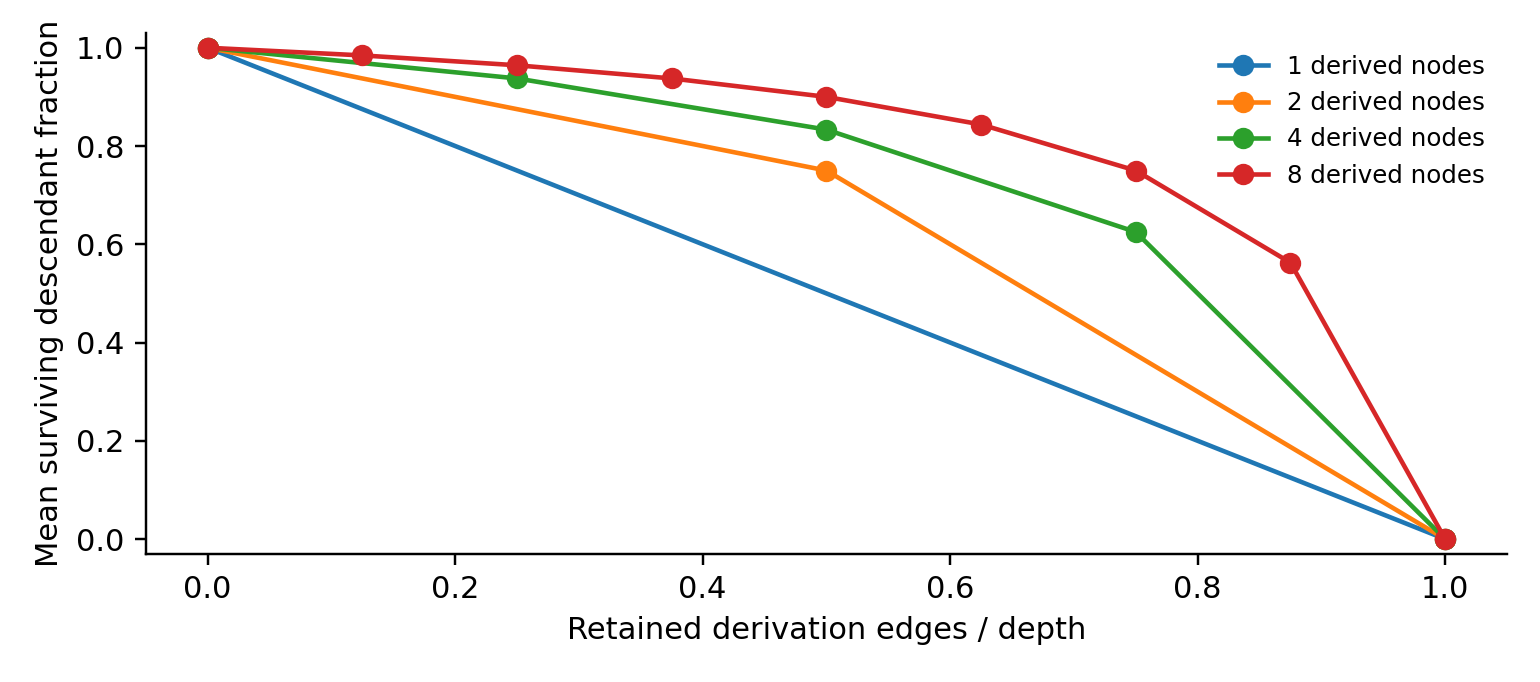
\includegraphics[width=.78\linewidth]{../figures/chain-sensitivity.png}
\caption{Preserved abstract chain enumeration, recomputed against all 278 masks. Means average equally weighted masks with the same depth and retained-edge count; they are not empirical probabilities of production failures.}
\label{fig:sensitivity}\end{figure}

\subsection{Structural deletion and information retention}
All 560 deterministic runs complete and verify. Four held-out complete-attack cases contain 11 target originals, eight unrelated facts and four lookup tasks. Source-only deletion exposes all four cases. Direct invalidation leaves 7/11 target originals accessible and exposure in 3/4. Cascade removes all target originals but retains 2/8 unrelated facts and succeeds on 1/4 lookups. Both reconstruction variants retain 8/8 facts and succeed on 4/4 lookups with no exposure (Table~\ref{tab:expanded}). Guarded and unguarded reconstruction are equal on every scored complete-attack metric across all 16 families.

\begin{table}[H]\centering\small
\begin{tabular}{lrrrrr}
\toprule
Strategy & Physical & Accessible & Exposed & Benign facts & Lookups\\\midrule
\multicolumn{6}{l}{\textit{Complete lineage}} \\
Source only & 11/11 & 11/11 & 4/4 & 8/8 & 4/4 \\
Keyword & 11/11 & 0/11 & 0/4 & 2/8 & 1/4 \\
Direct & 7/11 & 7/11 & 3/4 & 6/8 & 3/4 \\
Cascade & 0/11 & 0/11 & 0/4 & 2/8 & 1/4 \\
Re-derive & 0/11 & 0/11 & 0/4 & 8/8 & 4/4 \\
Quarantine & 0/11 & 0/11 & 0/4 & 2/8 & 1/4 \\
Guarded re-derive & 0/11 & 0/11 & 0/4 & 8/8 & 4/4 \\
\addlinespace[3pt]
\multicolumn{6}{l}{\textit{Marked gaps}} \\
Source only & 11/11 & 11/11 & 4/4 & 8/8 & 4/4 \\
Keyword & 11/11 & 0/11 & 0/4 & 2/8 & 1/4 \\
Direct & 11/11 & 11/11 & 4/4 & 8/8 & 4/4 \\
Cascade & 11/11 & 11/11 & 4/4 & 8/8 & 4/4 \\
Re-derive & 11/11 & 11/11 & 4/4 & 8/8 & 4/4 \\
Quarantine & 11/11 & 0/11 & 0/4 & 0/8 & 0/4 \\
Guarded re-derive & 11/11 & 0/11 & 0/4 & 0/8 & 0/4 \\
\addlinespace[3pt]
\multicolumn{6}{l}{\textit{Silent gaps}} \\
Source only & 11/11 & 11/11 & 4/4 & 8/8 & 4/4 \\
Keyword & 11/11 & 0/11 & 0/4 & 2/8 & 1/4 \\
Direct & 11/11 & 11/11 & 4/4 & 8/8 & 4/4 \\
Cascade & 11/11 & 11/11 & 4/4 & 8/8 & 4/4 \\
Re-derive & 11/11 & 11/11 & 4/4 & 8/8 & 4/4 \\
Quarantine & 11/11 & 5/11 & 3/4 & 6/8 & 3/4 \\
Guarded re-derive & 11/11 & 5/11 & 3/4 & 6/8 & 3/4 \\
\addlinespace[3pt]
\bottomrule
\end{tabular}

\caption{Study B held-out attack conditions, four families each. Physical/accessible counts refer to 11 original target artifacts; exposed cases have denominator four, unrelated facts eight and lookups four. A quarantined original can remain physically stored while inaccessible. These are deterministic outcomes, not attack-success rates.}
\label{tab:expanded}\end{table}

Marked partial lineage changes this conclusion. Recorded cascade and unguarded reconstruction leave 11/11 target originals accessible, exposing all four cases. Guarded retrieval blocks them, yet also loses all eight unrelated facts and all four lookups. These contaminated originals remain physically stored: containment is not deletion.

With silent loss, the guard still admits contaminated context in families f14, f15 and f16. Five of 11 originals are accessible, exposure is 3/4, unrelated-fact retention 6/8 and lookup success 3/4. A surviving clean root conceals the lost malicious branch. Keyword filtering yields no exposure across these attack conditions, but retains only 2/8 facts and depends on knowing the exact canary.

Never-exposed held-out controls retain 8/8 unrelated facts and 4/4 lookups under all strategies. Clean deletion controls show that mixed-information loss is not specific to malicious text. Development cases are preserved, not discarded: complete attack exposure is 0/12 for both cascade and guarded reconstruction; marked and silent exposure is 9/12 for cascade, versus 0/12 and 3/12 for guarded reconstruction. These fixed fixtures do not establish a population distribution.

\subsection{Exploratory local-model behavior}
Study C records 74 actual chat requests and 74 HTTP-200 responses. Qualification succeeds 4/4; all 70 planned probes are valid, with zero invalids. Each saved probe database contains the legitimate ticket, yielding 70/70 exact legitimate effects. There are zero exact attacker proposals and zero exact attacker effects in 42 eligible observations. No probe response text contains the literal canary.

Every strategy scores 10/10 legitimate effects and 0/6 attacker effects. There is therefore no behavioral separation between MemoryFence and its baselines. Context exposure in Study B cannot be promoted to an executed attack in Study C, and the latter's zero effects cannot retroactively certify Study B's exposed memories as safe. The literal task and small model may reduce sensitivity to this payload; the design cannot distinguish a broadly robust model from a narrowly ineffective attack.

Earlier exploratory populations also remain relevant. The original 28-cell 0.5B pilot failed its legitimate tool-utility control, making absent attacks uninterpretable as protection. Separate follow-up accessions include native-contract failures and 11 source-alive exact objective effects in a different schema-controlled condition. Those effects are not post-deletion successes and are not pooled with the final studies. Their preservation prevents interface revisions from erasing unfavorable evidence.

\section{Discussion and Limitations}
\subsection{A common dependency can defeat multiple controls}
Deletion and historical author filtering depend on the same recorded paths. A missing edge can both disconnect a descendant from deletion reach and remove evidence that would have excluded it. The linear-chain counterexample is simple, but the mixed-source expansion shows why fail-closed treatment of visible uncertainty does not solve silent missingness. An admitted memory is merely consistent with the available evidence. Systems should expose that distinction rather than labeling all admitted context trustworthy.

\subsection{Reconstruction benefits are conditional}
Complete-lineage reconstruction recovers unrelated information that cascade discards. The guard does not improve that condition over existing DS4. Under visible gaps, conservative containment trades away legitimate facts; under silent gaps, it can retain those facts alongside contamination. Across all five held-out controls, guarded-minus-unguarded reconstruction benign retention has family-macro delta $-0.25$, with family range $[-0.40,-0.20]$. This unfavorable aggregate remains alongside the conditional positive result.

Reconstruction here uses structured union, not semantic rewriting. We do not establish faithful recovery of preferences, complex reasoning chains or natural-language summaries. The tested guarded-input rejection path is an implemented safeguard, not a measured explanation for the complete-lineage benefit. Future work should isolate scheduling reach, input selection and generation quality as separate factors.

\subsection{External validity and uncertainty}
The benchmark has 16 authored structural families, below earlier planning targets, and only four held-out families. Source kinds are not independent domains. Partial loss is seeded edge omission, not realistic correlated logging failure, incorrect ancestry or malicious metadata forgery. There are no long-delay deployments, arbitrary concurrency guarantees or learned retrieval systems.

The model studies use small quantized Qwen artifacts and narrow exact objectives. Study A behavior is complete-lineage only; Study C uses one known family, deterministic contexts and a task that does not require memory. Seeds and temperature zero do not guarantee deterministic inference or independent samples. No human-validated semantic outcome labels or broad adaptive attack search are provided.

Zero observed effects does not establish a zero risk or a generally effective defense. A valid structured response can still contain contaminated text; a stored canary need not cause an action. No confidence interval based on 42 independent attacks is justified. The framework's strongest conclusion concerns the tested implementations and explicit counterexamples, not universal vulnerability or safety.

\subsection{Reliability of the measurement software}
Results depend on the evaluator as well as the agent. Full-grid validation rejects duplicate/missing strategy substitutions, inconsistent metadata, nonfinite ratios and behavioral values in deterministic records. Independent verification reads raw journals and sandbox rows. These checks reduce some errors without excluding shared conceptual mistakes or dishonest inference-host records.

A new evidence-verification run for this manuscript recomputes original analyses, all graph masks, expanded records, saved deterministic reproduction and the local-model accession without new inference. Software tests separately exercise ACL denial, provenance validation, reconstruction, rollback, transport failures and evidence corruption. Test success and source coverage describe software verification, not scientific validation or defense efficacy.

\section{Conclusion}
MemoryFence shows how the operational fate of agent memory depends on recorded ancestry. In the tested chains, missing links preserve derived instructions after source deletion; in the structural expansion, complete lineage enables unrelated-fact recovery, visible gaps impose containment costs and silent gaps can evade the guard. Qualified models nevertheless produce no exact attacker effect in the final bounded conditions, with no behavioral advantage for the guarded strategy.

The appropriate next step is a separately versioned study with fresh semantic memory generation, realistic memory-dependent tasks, independent scenario families, multiple models and explicit semantic adjudication. No new experiment should be silently added to an original denominator. The present contribution is a reproducible, inspectable account of conditional failures and measurement boundaries.

\section*{Author Contributions and AI Assistance}
Yug Amol More initiated the research direction, guided the experimental design and scenario objectives, oversaw framework development, coordinated evaluation, and reviewed the findings and manuscript. The project was conducted independently, without human research collaborators or a research supervisor. AI assistance was used in software development and manuscript drafting.

\section*{Ethics and Availability}
Sources, identities and tickets are synthetic. Canary addresses use a reserved invalid domain, and tools affect only local sandbox rows. The completed runs used explicitly free local or Colab resources, without paid APIs or external messaging. Research journals retain deleted-source content intentionally; privacy erasure from evidence is outside the study. No project license is established, and public repository access does not grant unrestricted reuse. Code and evidence are available at \url{https://github.com/Yug-More/memoryfence}.

\clearpage
\begingroup\raggedright
\bibliographystyle{plainnat}
\bibliography{references}
\endgroup
\clearpage
\appendix
\section{Reproducibility and Evidence Map}\label{app:artifacts}
All counts have distinct units (Table~\ref{tab:units}). The manuscript's generator verifies preserved evidence without a model and writes new tables and a provenance ledger only under \path{paper/revised/generated/}. It checks the original 53-file and expanded 12-file inventories plus the 46-entry prior-finalization inventory without altering them. Source and output hashes identify the supplied bytes. PDF metadata may vary across compiler runs.

\begin{table}[H]\centering\small
\begin{tabular}{>{\raggedright\arraybackslash}p{.25\linewidth}>{\raggedright\arraybackslash}p{.64\linewidth}}\toprule
Evidence & Unit and archive location\\\midrule
Study A qualification & 24 actual replies; \path{experiments/2026-10-25-bounded/final-qualification.zip.xz}\\
Study A chains/state & Six generated chains, 12 transformation replies, 108 declared plus 36 off-protocol views; \path{paired-state-study.zip.xz} in the same accession\\
Study A behavior & 36 actual responses, 18 attack episodes, complete lineage only; same paired-state archive\\
Graph sensitivity & 278 abstract masks; \path{paper/generated/chain-sensitivity.json}\\
Study B & 560 deterministic runs, no inference; \path{experiments/2026-11-07-expanded/expanded-v1.zip.xz}\\
Study C & 4 qualification plus 70 real probes; \path{experiments/2026-11-09-model-followup/model-followup.zip.xz}\\\bottomrule
\end{tabular}
\caption{Evidence populations. Records from different accessions are not pooled.}
\label{tab:units}\end{table}

Study A execution revision is \texttt{e5dcc3c}; Study B uses \texttt{4a430fa}; Study C uses \texttt{4a82416}. The pre-refinement main is \texttt{135fc025}. Study A's pinned execution used a task-last transport permutation; the current explicit task-last adapter has request-equivalence tests, rather than being falsely described as the historical runner. The shared 1.5B model digest is:
\begin{quote}\footnotesize
\texttt{65ec06548149b04c}\allowbreak\texttt{096a120e4a6da9d4}\allowbreak\texttt{017ea809c91734ea}\allowbreak\texttt{5631e89f96ddc57b}
\end{quote}

Independent verifiers are \path{scripts/research/verify_final.py}, \path{verify_expanded.py} and \path{verify_model_followup.py} in that directory. Study C's archive contains \path{http.jsonl}, \path{qualification.json}, \path{probes.json} and per-probe result/system/ground-truth SQLite files. Study B provides \path{records.json} and per-strategy snapshots. The 36 off-protocol views and native failures remain in their original accessions.

From the repository root, the model-free manuscript workflow is:
\begin{quote}\small\ttfamily
uv sync --frozen\\
uv run --frozen python paper/revised/generate.py\\
mkdir -p /tmp/memoryfence-paper-build\\
tectonic --keep-logs --outdir /tmp/memoryfence-paper-build \textbackslash{}\\
\hspace*{1em}paper/revised/main.tex
\end{quote}
Tectonic 0.17.0 is an optional free compiler; its first run can fetch TeX resources. The application lockfile does not include TeX or plotting tools. Full commands, archived verification results, manuscript-specific checks and software-validation logs are indexed in \path{docs/MANUSCRIPT_VERIFICATION_2026_11_18.md}. The historical manuscripts remain separate and are not retrospectively rewritten to include later findings.
\end{document}
